\chapter{Proposed Methodology}

The proposed virtual assistant system is designed to streamline various tasks within a banking application, significantly enhancing efficiency and user experience. In the banking sector, employees often spend considerable time manually processing transactions and handling customer requests, which can be tedious and time-consuming. Our virtual assistant can drastically reduce this time. The system employs a large language model (LLM) to understand user queries and generate appropriate functions. These functions are then executed by an action engine, which processes the results and returns them in a JSON format. The results are subsequently displayed to the user in an easily understandable manner, making banking operations faster and more efficient. This transformation can decrease task completion time from several hours to mere minutes, thereby significantly improving productivity.

\vspace{1.5mm}

\begin{figure}[h!]
    \centering
    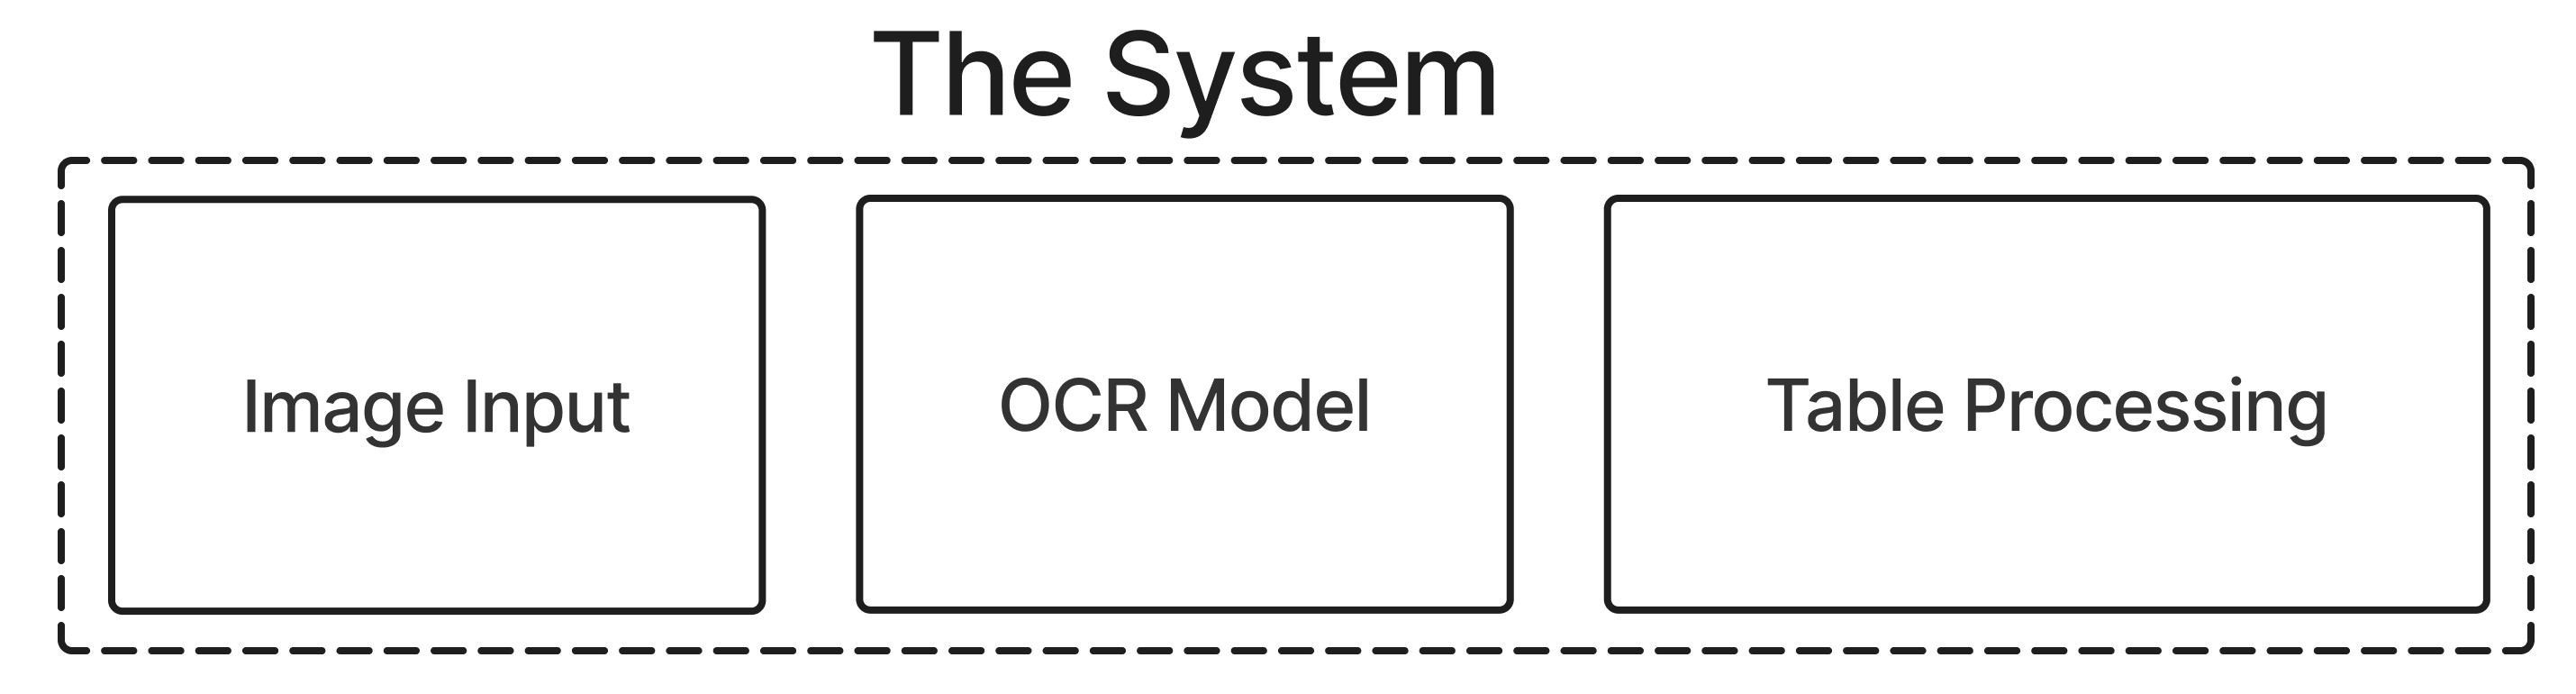
\includegraphics[width=0.8\textwidth]{Images/lit_review/main_components_of_MP.jpg}
    \caption{Main components of the system}
\end{figure}

\noindent
As per the overall literature survey and research, it is evident that the modular approach for system building is the best. A modular design for the system is illustrated using Figure 3.1, where the idea of modules would be the building blocks for the system and they serve the purpose of ease of development and modification. The explanation for each block is as follows: 

\clearpage

\begin{enumerate}
    \item Image Input: Users can edit this module to make the system work with any input type like PDF, at the end the system should work on a single image at a time.
    \item OCR Model: To make the system more robust to different handwritings this module can be edited or replaced with a better model weights file. 
    \item Table Processing: Users can edit this module to process tables of different formats (rows and columns).
\end{enumerate}.

\section{Overview of the Proposed System}

\noindent The core objective of this project is to create a highly intuitive and user-friendly software tool that facilitates the recognition of handwritten numbers and seamlessly converts them into structured CSV files. By employing Optical Character Recognition as its primary technology, the software allows users to capture a picture of the front page of an answer script using a simple camera as input. The captured image cells are then skillfully processed through a specialized Convolutional Neural Network Model, skillfully built using TensorFlow, to ensure precise and reliable conversion of handwritten marks into digital text.

\noindent This novel approach serves as a powerful solution to the challenges faced during manual data entry, offering educators and researchers an efficient means to transform vast quantities of handwritten data into easily manageable and structured CSV files. With the integration of OCR and CNN technologies, this software tool not only enhances the speed and accuracy of digit data processing but also paves the way for informed decision-making, data analysis, and optimal results across diverse domains.

\noindent Upon extracting the marks and converting the handwritten data into digital text, the software proceeds to process the information, generating a comprehensive CSV sheet that accurately reflects the content of the original answer scripts. This automated approach saves time and minimizes errors typically associated with manual data entry. The resulting CSV sheet is structured, organized, and ready for data analysis, providing the teachers with actionable insights to optimize their teaching approaches and interventions.

\clearpage

\begin{figure}[htbp]
  \centering
  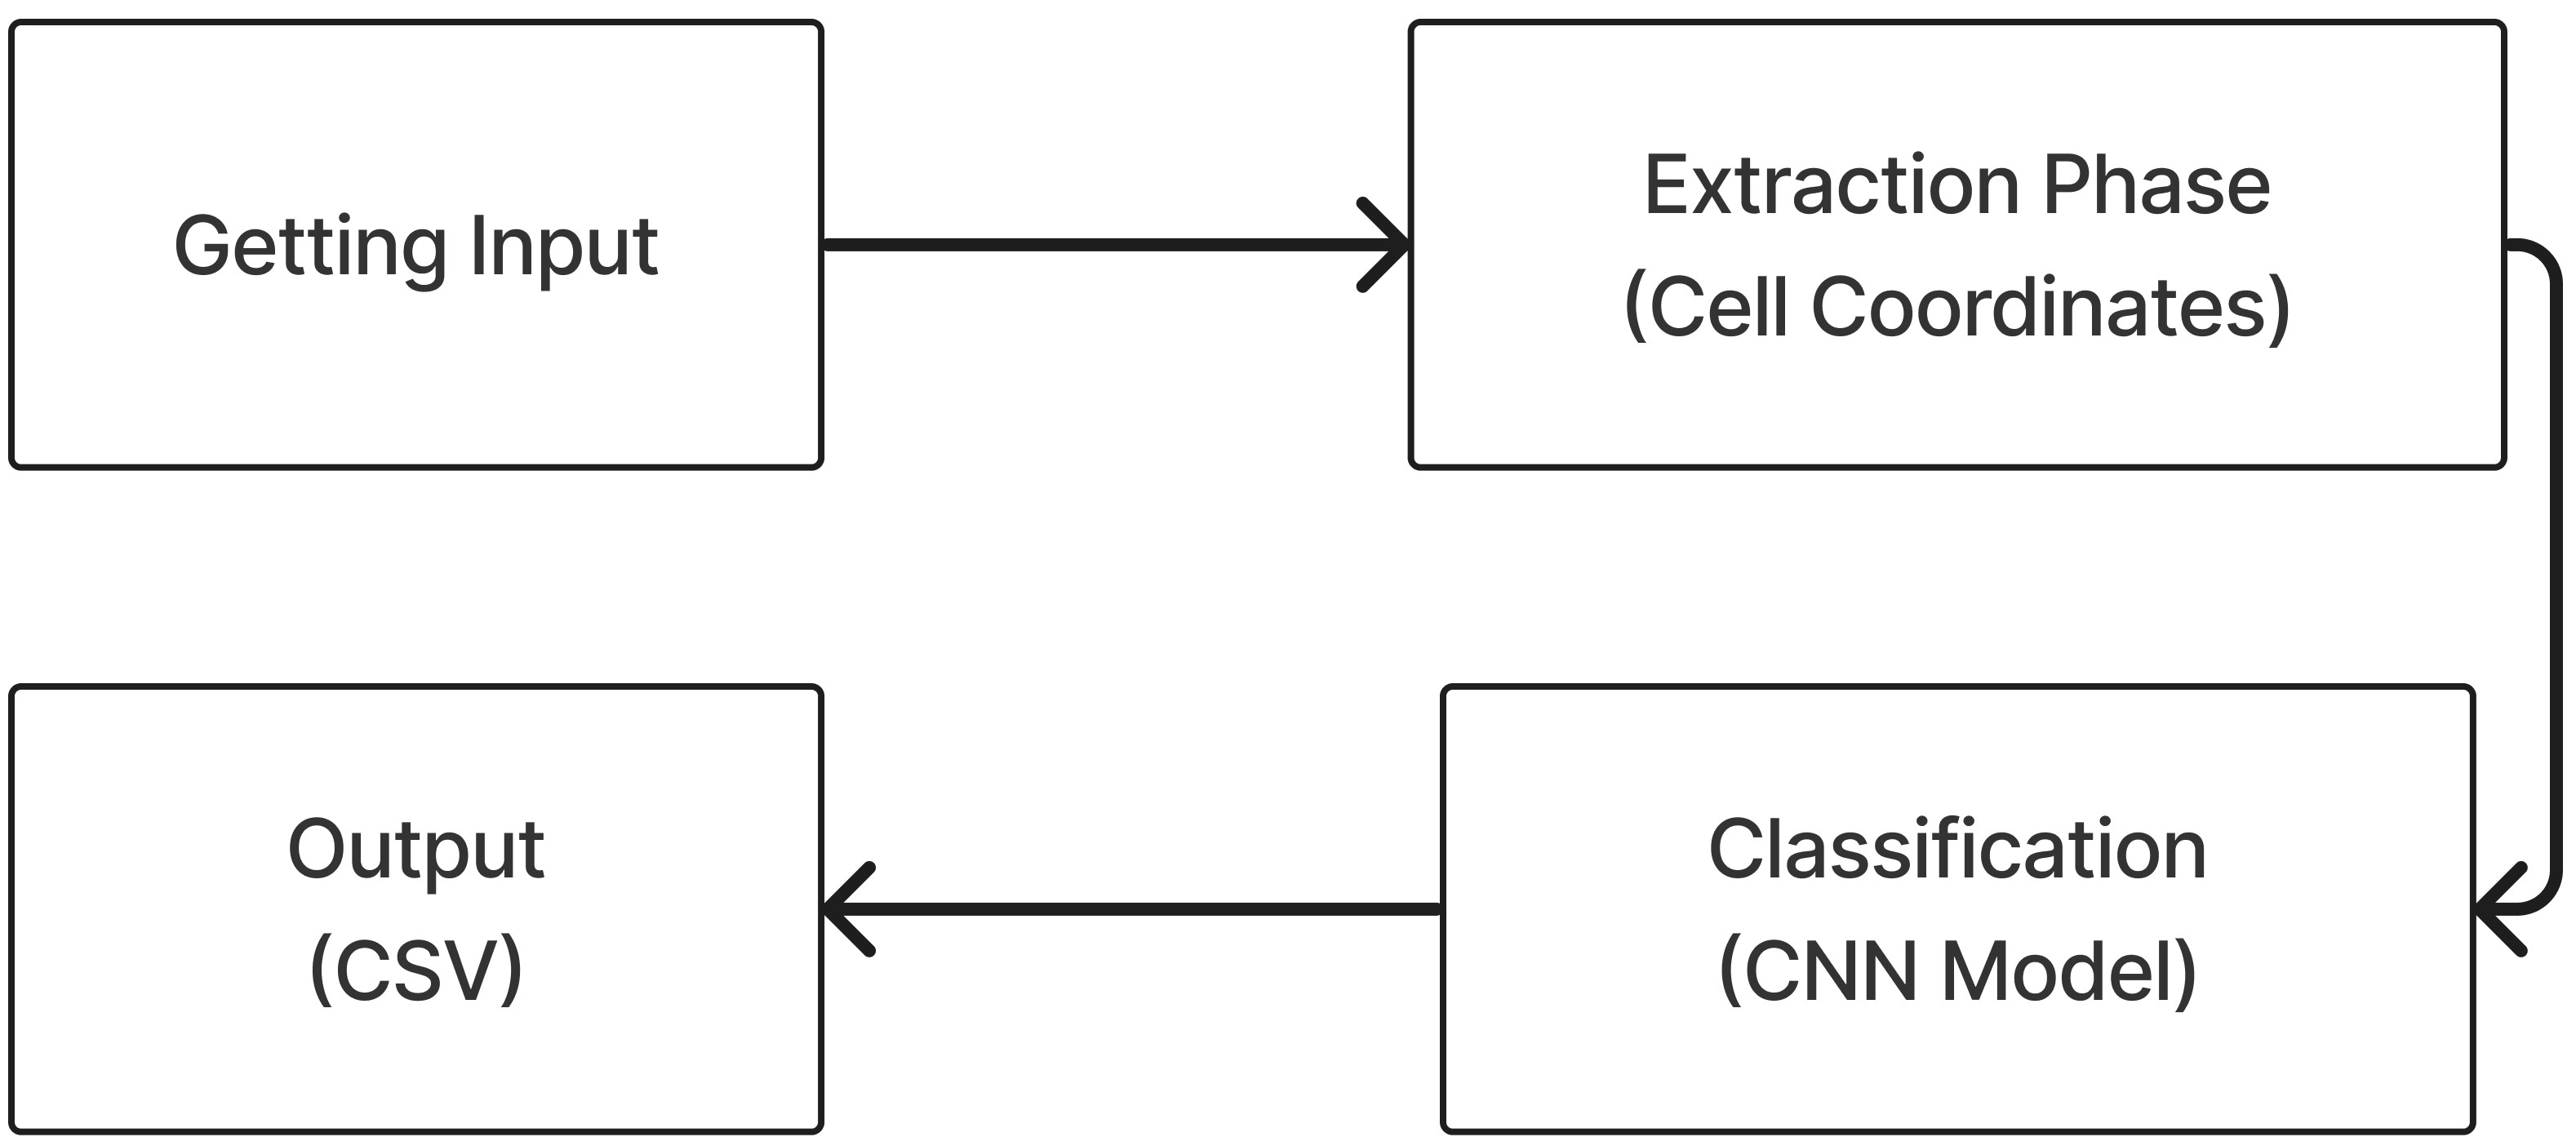
\includegraphics[width=0.9\textwidth]{Images/prop_sys/overview_prop_sys.jpg}
  \caption{Overview of proposed system}
\end{figure}

\section{Detailed Description Of The System}

\noindent
The application features a professional and efficient user interface, developed using HTML and Flask. Designed to enhance interactivity and performance, this interface serves as the entry point for teachers to interact seamlessly. A camera icon in the center enables users to quickly open the camera and capture images of answer scripts, streamlining the process. This intuitive design fosters a professional environment, empowering teachers with a streamlined approach to their tasks.

\noindent The input images are processed by the img2table library for table recognition. Figure 3.3 shows the recognized table structure.

\begin{figure}[h!]
    \centering
    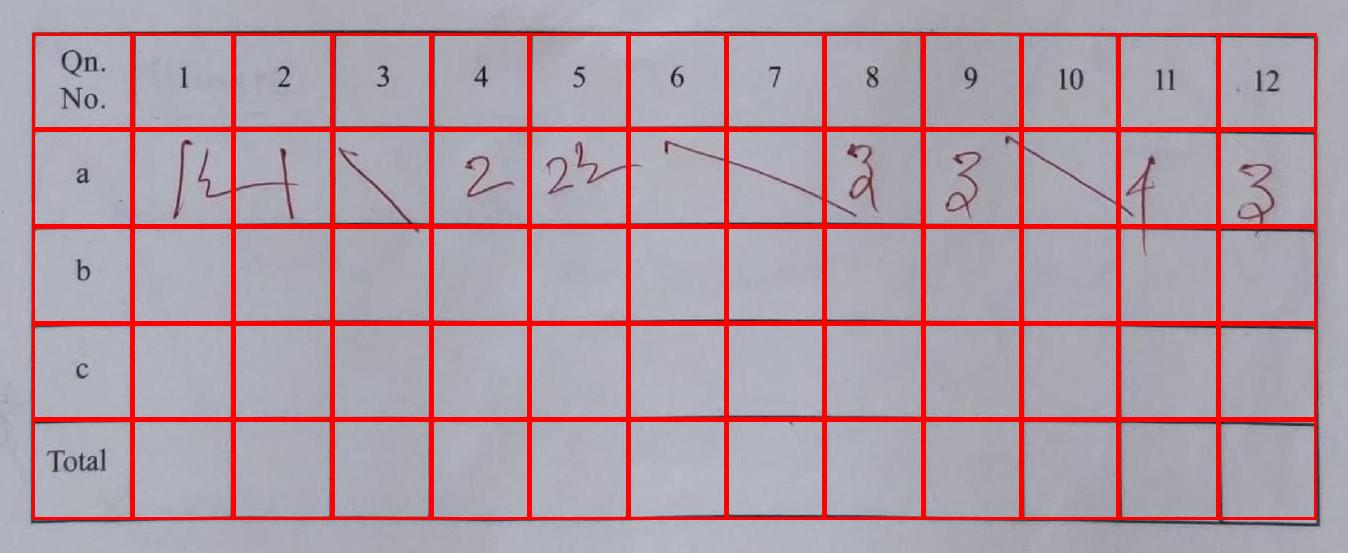
\includegraphics[width=0.8\textwidth]{Images/prop_sys/Img_with_redlines.jpg}
    \caption{Sample Output Of Table Detection Process}
\end{figure}

\clearpage

\noindent \textbf{The table processing phase of the system is designed by taking a sample of the answer scripts of SJCET Palai.} SJCET college answer script is in the format of a horizontal table that consists of question number written on the first row (13 cells), the first column is a place-holder for headings (Qn. No. and Total), and possible divisions of questions in each question number (A, B, C). In overall, the table has the total number of cells and the total number of mark cells as 65 and 36 respectively.\\ 

\noindent The data preprocessing phase for the \textbf{mark table of SJCET Palai} answer script isolates the 36 mark cells, which may or may not contain the marks written on them. For this, the first and the last columns, as well as the first row are removed.

\noindent For extracting cells from the image and converting the extracted cells to its digital text, the model makes use of the img2table library and an OCR engine respectively, and for executing the whole process, there are two methods: one involves the use of \textbf{img2table library}, and the other involves \textbf{extracting cell coordinates}. A detailed explanation and side-by-side comparison are written in paragraphs and with a comparison Table 3.1 respectively.\\

\noindent Method 1: \textbf{img2table library}\\

\noindent In this method, the system uses the img2table library in combination with PaddleOCR (built-in to the same library) to detect the table, extract coordinates of table cells, and perform OCR on each extracted cell using PaddleOCR. These three processes are executed using an attribute called on the input image, which is converted to the proprietary document type of the library.\\

% \begin{figure}[h!]
%   \centering
%   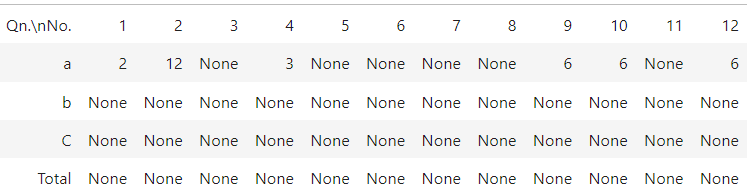
\includegraphics[width=0.8\textwidth]{Images/prop_sys/paddle_ocr_output.png}
%   \caption{DataFrame Output of img2table library method using PaddleOCR}
% \end{figure}


\begin{table}[ht]
  \centering
  \footnotesize
  \begin{tabular}{|c|c|c|c|c|c|c|c|c|c|c|c|c|}
  \hline
  Qn. No. & 1 & 2 & 3 & 4 & 5 & 6 & 7 & 8 & 9 & 10 & 11 & 12 \\
  \hline
  a & 2 & 12 & None & 3 & None & None & None & None & 6 & 6 & None & 6 \\
  \hline
  b & None & None & None & None & None & None & None & None & None & None & None & None \\
  \hline
  c & None & None & None & None & None & None & None & None & None & None & None & None \\
  \hline
  Total & None & None & None & None & None & None & None & None & None & None & None & None \\
  \hline
  \end{tabular}
  \caption{DataFrame output of img2table library method using PaddleOCR}
\end{table}


\noindent  Consequently, the programmer does not have explicit control over the individual stages to meet specific requirements. The resulting DataFrame (shown in Table 3.1) is then post-processed to remove the first column and the first and last rows.\\

% \vspace{1.5mm}

\noindent Method 2: \textbf{Cell Coordinates Extraction}

\vspace{1mm}

\noindent In this method, the system extracts only the cell coordinates using the img2table library. The extracted table cells are stored in an ordered dictionary.

\vspace{1mm}

\noindent \textit{OrderedDict is a dictionary subclass in Python that maintains the order of key-value pairs. Even if the value of a key is modified, the order of the keys remains unchanged. In contrast, a regular dictionary does not guarantee a specific order and may reorder the keys when their values are modified.}

\vspace{0.5mm}

\noindent In the ordered dictionary data structure, each key represents a single row of the mark table, so deleting a key is equivalent to removing a row from the table, thus deleting the first and last keys of the ordered dictionary. There is a  need to remove the first column (column with A, B, and C written) also, but it could be easily done after converting the presently existing cells to their DataFrame format.

\noindent From the two methods above, the second method was chosen as it has the following benefits (shown in Table 3.2).

\begin{table}[h!]
  \centering
  \renewcommand{\arraystretch}{1.2}
  \begin{tabular}{|l|p{4.5cm}|p{4.5cm}|}
      \hline
      \textbf{ } & \textbf{Cell Coordinates Extraction Method} & \textbf{PaddleOCR Method} \\
      \hline
      \textbf{Speed} & Very fast as it works with built-in data structures. & Slow, as it runs the big PaddleOCR engine. \\
      \hline
      \textbf{Programmer's Control} & Highly controllable & No control \\
      \hline
      \textbf{Ease of programming} & Difficult & Easy \\
      \hline
      \textbf{Ease of understanding} & Medium & Easy Outwards, Internal working codes are complex.\\
      \hline
      \textbf{Time taken} & 13 seconds for 5 papers & 44 seconds for 5 papers \\
      \hline
  \end{tabular}
  \caption{Comparison of Table Processing Methods}
\end{table}

\clearpage

\noindent Once the ordered dictionary is processed, the remaining table cells are cropped based on these coordinates and forwarded to the CNN model. Table 3.3 depicts the classification time taken by the CNN model for each individual image, showcasing the exceptional speed and efficiency of the model. The CNN model is specifically designed with a minimum number of layers to make it perform efficiently on smaller images. This way, it ensures that the proposed system prioritizes speed without compromising accuracy. It boasts an impressive capability to process five images in a mere 13 seconds, showcasing its remarkable performance.

\begin{table}[htbp]
    \centering
    \begin{tabular}{|c|c|}
        \hline
        Image Count & Time per step (ms) \\
        \hline
        1 & 23 \\
        2 & 18 \\
        3 & 17 \\
        4 & 17 \\
        5 & 16 \\
        6 & 16 \\
        7 & 16 \\
        8 & 23 \\
        9 & 20 \\
        10 & 19 \\
        \hline
        Average time: & 18.5 \\
        \hline
    \end{tabular}
    \caption{Classification time taken for CNN OCR Model Version 1}
\end{table}

\noindent The output after the classification and some processing is a DataFrame. This DataFrame is post-processed to remove the first column using a \textit{Pandas} function.\\

\noindent The final dataframe will be converted to a NumPy array for flattening the DataFrame; And the two-dimensional array is flattened column-wise to get the marks corresponding to each sub-division (1A, 1B, ..., 12B, 12C). The output is a one-dimensional array that represents the marks scored by a student in individual questions.

\clearpage

\noindent The flattened array is incorporated into a dictionary to store the marks of individual students. Following this step, additional coding is applied for post-processing, which includes the removal of columns with identical entries and adding the columns \textit{Roll No.} and \textit{Name} to the left side of the DataFrame. This DataFrame is then converted to CSV format without the index values.\\

% \begin{figure}[h!]
%     \centering
% {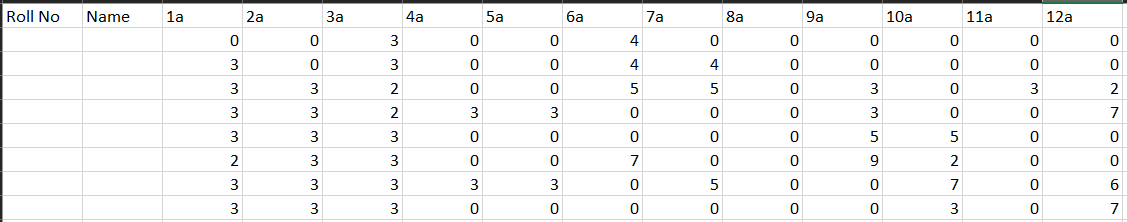
\includegraphics[width=1\textwidth]{Images/prop_sys/csv_output.png}}
%   \caption{Output CSV File}
% \end{figure}

\begin{table}[ht]
  \centering
  \small
  \begin{tabular}{|c|c|c|c|c|c|c|c|c|c|c|c|c|c|}
  \hline
  Roll No & Name & 1a & 2a & 3a & 4a & 5a & 6a & 7a & 8a & 9a & 10a & 11a & 12a \\
  \hline
   &  & 0 & 0 & 3 & 0 & 0 & 4 & 0 & 0 & 0 & 0 & 0 & 0 \\
   \hline
   &  & 3 & 0 & 3 & 0 & 0 & 4 & 4 & 0 & 0 & 0 & 0 & 0 \\
   \hline
   &  & 3 & 3 & 2 & 0 & 0 & 5 & 0 & 0 & 3 & 0 & 3 & 2 \\
   \hline
   &  & 3 & 3 & 2 & 3 & 3 & 0 & 5 & 5 & 3 & 0 & 0 & 7 \\
   \hline
   &  & 3 & 3 & 3 & 0 & 0 & 0 & 0 & 0 & 5 & 5 & 0 & 0 \\
   \hline
  \end{tabular}
  \caption{Output CSV File}
\end{table}

\noindent The result is a refined CSV file that has the marks of all students (see a sample of output CSV in Table 3.4). The Roll Numbers and Names can be filled in by the faculty as roll numbers and names were not included in the work. Notably, this CSV file is automatically downloaded through the interface of the application, enabling seamless access to the finalized output on the local system.

\clearpage

\section{Block Diagram}

\subsection{Overall working of the system}

\noindent A camera is used to acquire the images and is stored in a list data structure. From each of these images, the table structure of the mark table is detected. This is done by a table detection algorithm, where the image is first cropped to half, and the table in the lower part is recognized by an optimized OpenCV algorithm (houghlinesP) then each cell coordinates are taken from the recognized table and is returned in an ordered dictionary.\\

\vspace{2 mm}

\noindent From this ordered dictionary, the first and last rows are removed by deleting the first and last keys of the ordered dictionary and transferring the cropped image using cell coordinates to the TensorFlow OCR model for classification. After the classification result is returned as a dataframe, from which the first column is removed. Now the dataframe is flattened to add the classified values to the marks dictionary. After this process runs on every image, this marks dictionary is transformed into a CSV file to obtain the final output.

\vspace{1 cm}

\begin{figure}[h!]
    \centering
    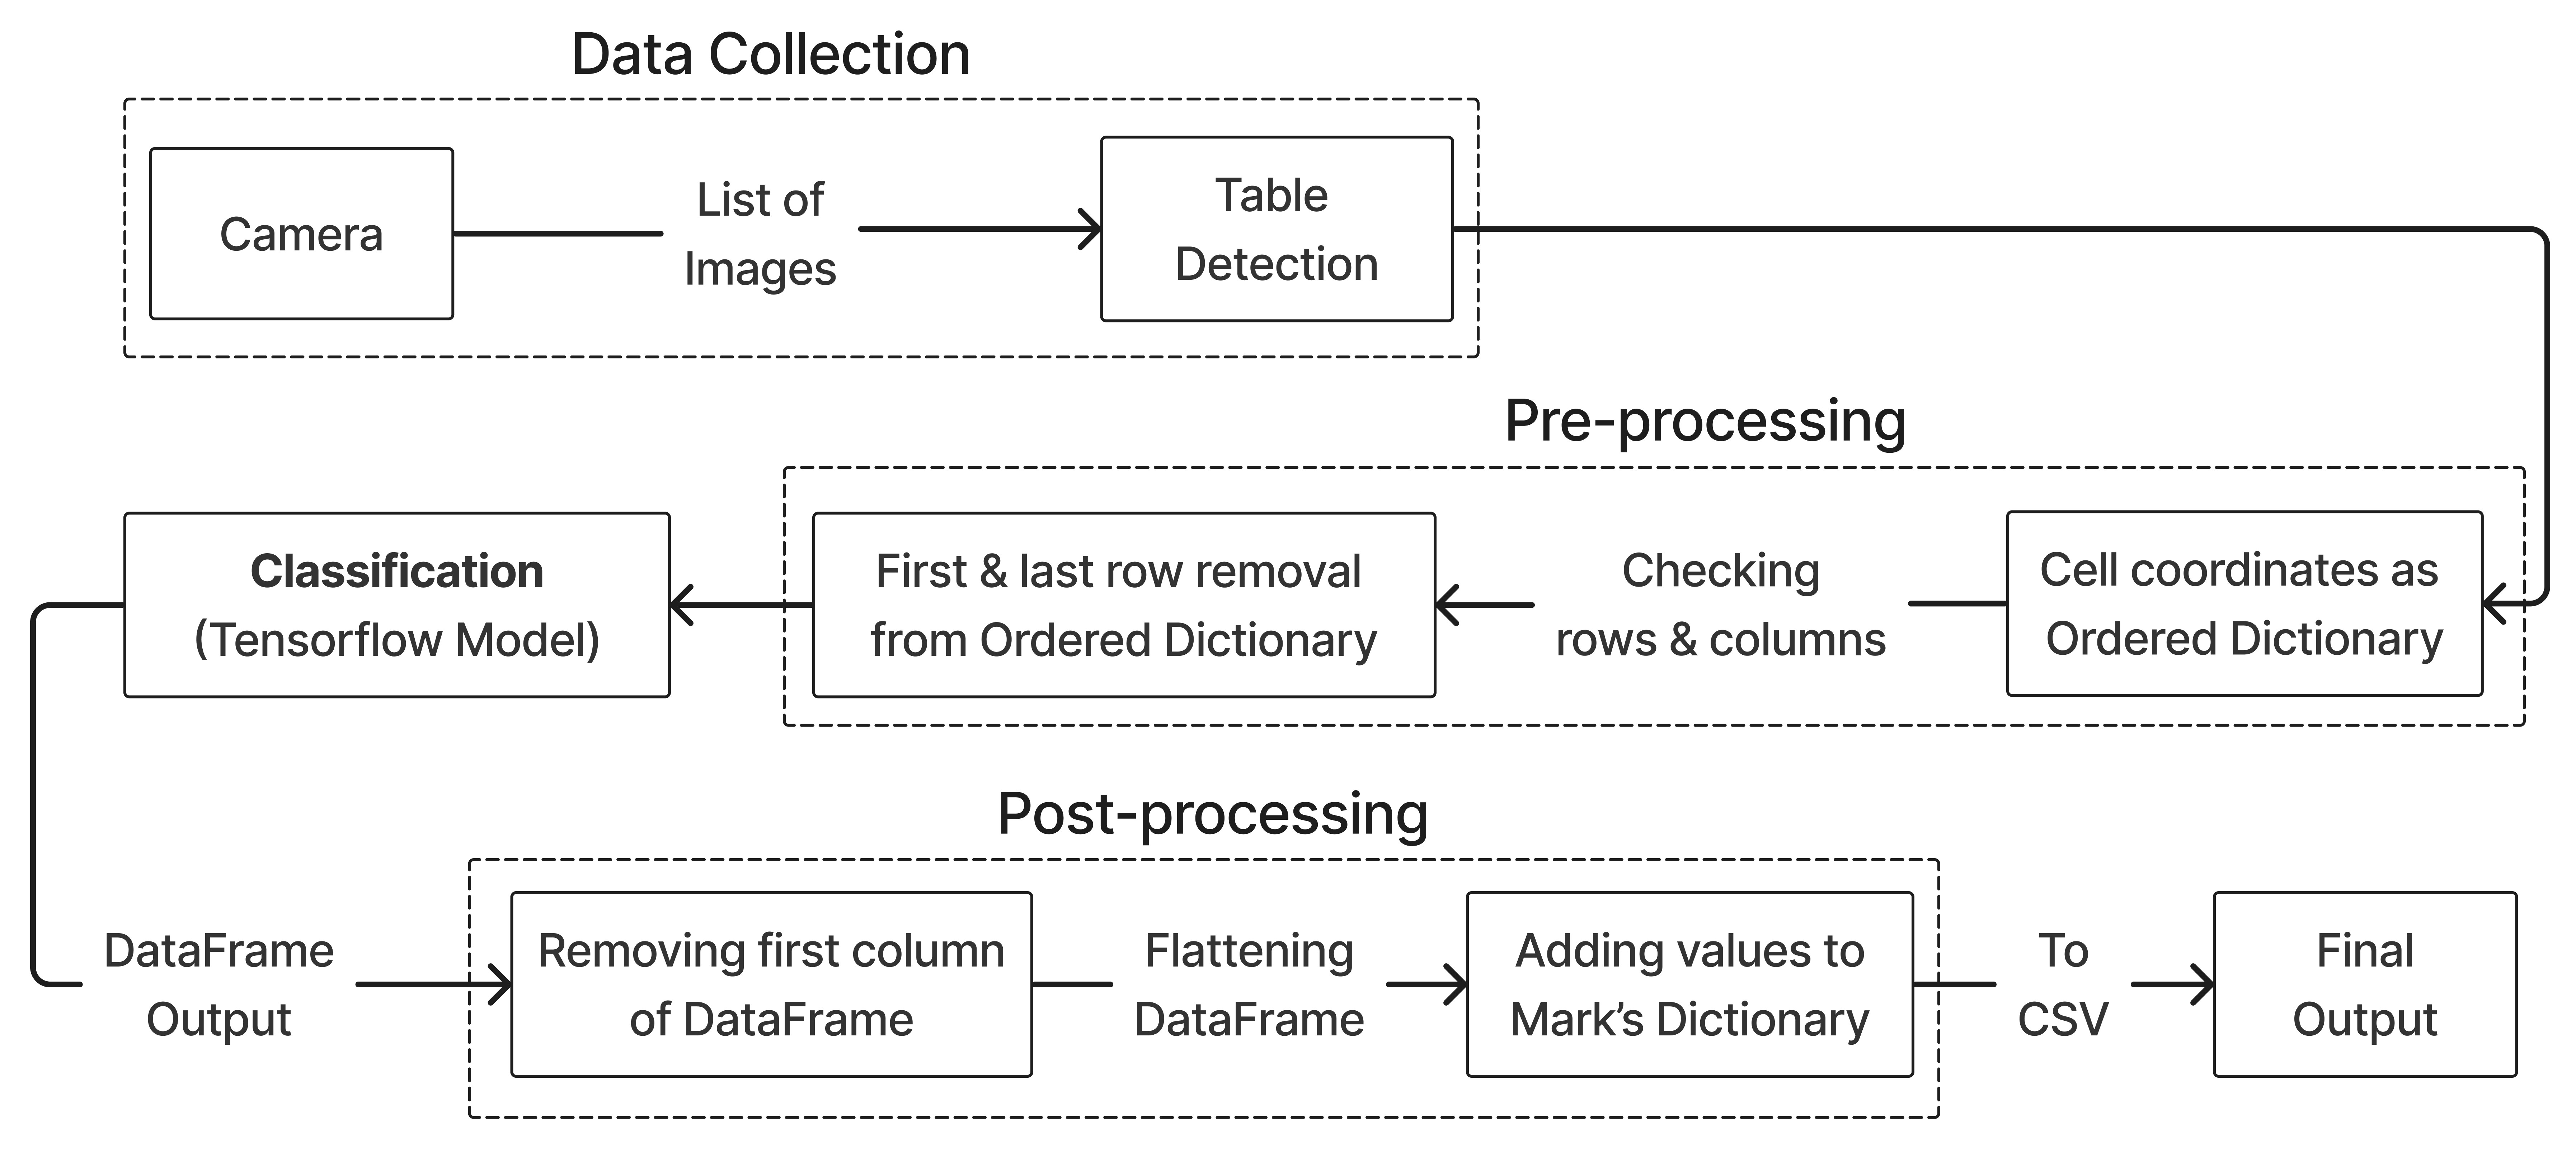
\includegraphics[width=\textwidth]{Images/Block_Diag/Flow_Diagram.jpg}
    \caption{Flow diagram of the proposed system}
\end{figure}

\clearpage

\subsection{Data Collection}

\noindent Initially, 614 images of data were collected privately. Understanding the fact that this data was insufficient to train the model properly, a collection of an additional 21,600 images from a public Kaggle dataset was made. As per the project requirements, the removal of image classes - numbers 8 and 9 from the public dataset reduced the public dataset image count from 21,600 images to 17,454 images. So the final dataset has a sum of 18,068 images.

\begin{figure}[h!]
    \centering
    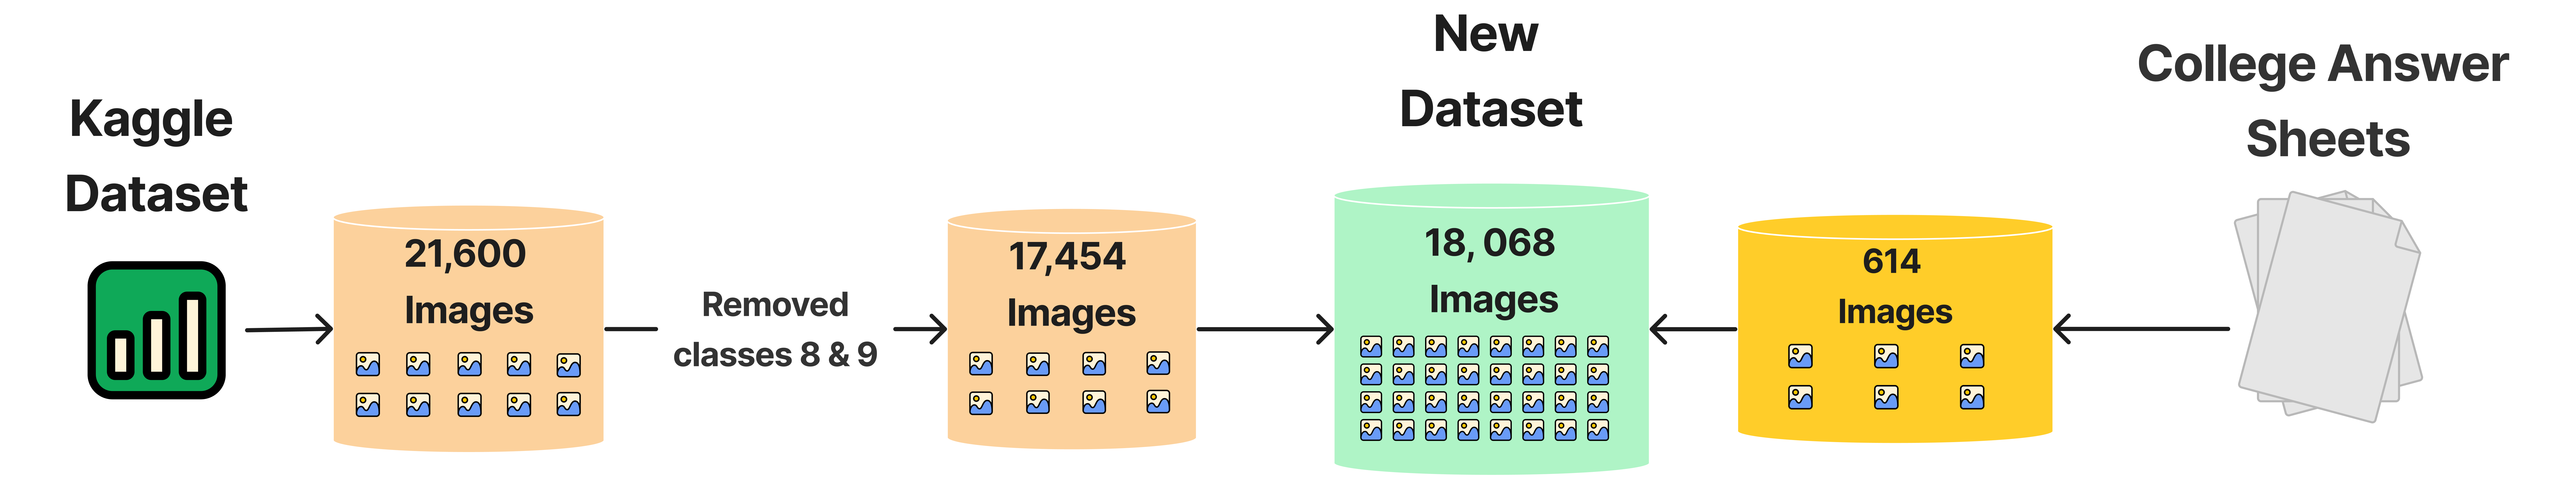
\includegraphics[width=\textwidth]
    {Images/Block_Diag/Dataset_Counts.png}
    \caption{Dataset Collection}
\end{figure}

\begin{figure}[h!]
    \centering
{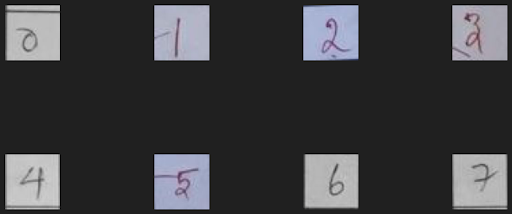
\includegraphics[width=0.7\textwidth]{Images/Block_Diag/Clg_ans_sheet.png}}
  \vspace{-15pt}
  \caption{Mark cells of private dataset}
\end{figure} 

\begin{figure}[htbp]
  \centering
  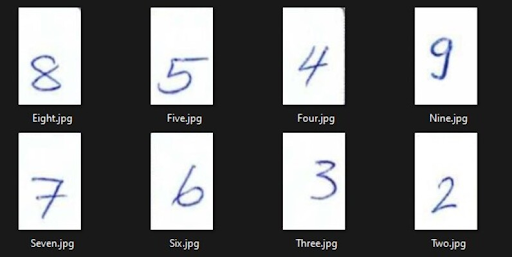
\includegraphics[width=0.7\textwidth]{Images/Block_Diag/Kaggle_Dataset_Header.png}
  \vspace{-15pt}
  \caption{Mark cells of the public dataset from Kaggle}
\end{figure}

\clearpage

\subsection{Data Pre-processing}

In the process of automated marks extraction, a crucial feature to be extracted is the mark associated with each cell of the table. A table extraction algorithm is employed to achieve this, which facilitates the extraction of marks from each cell when the entire table is detected. The algorithm operates by identifying the boundaries of the table and dividing it into square dimensions, representing individual cells.\\

\noindent Once the table is successfully detected and divided into cells, the marks extraction process begins. Each cell is isolated, and the algorithm focuses on extracting the mark contained within it. This is where the CNN model comes into play. The extracted cell is passed through the CNN model, which has been trained to classify and interpret the marks present within the cells accurately.\\  

\begin{figure}[h!]
    \centering
    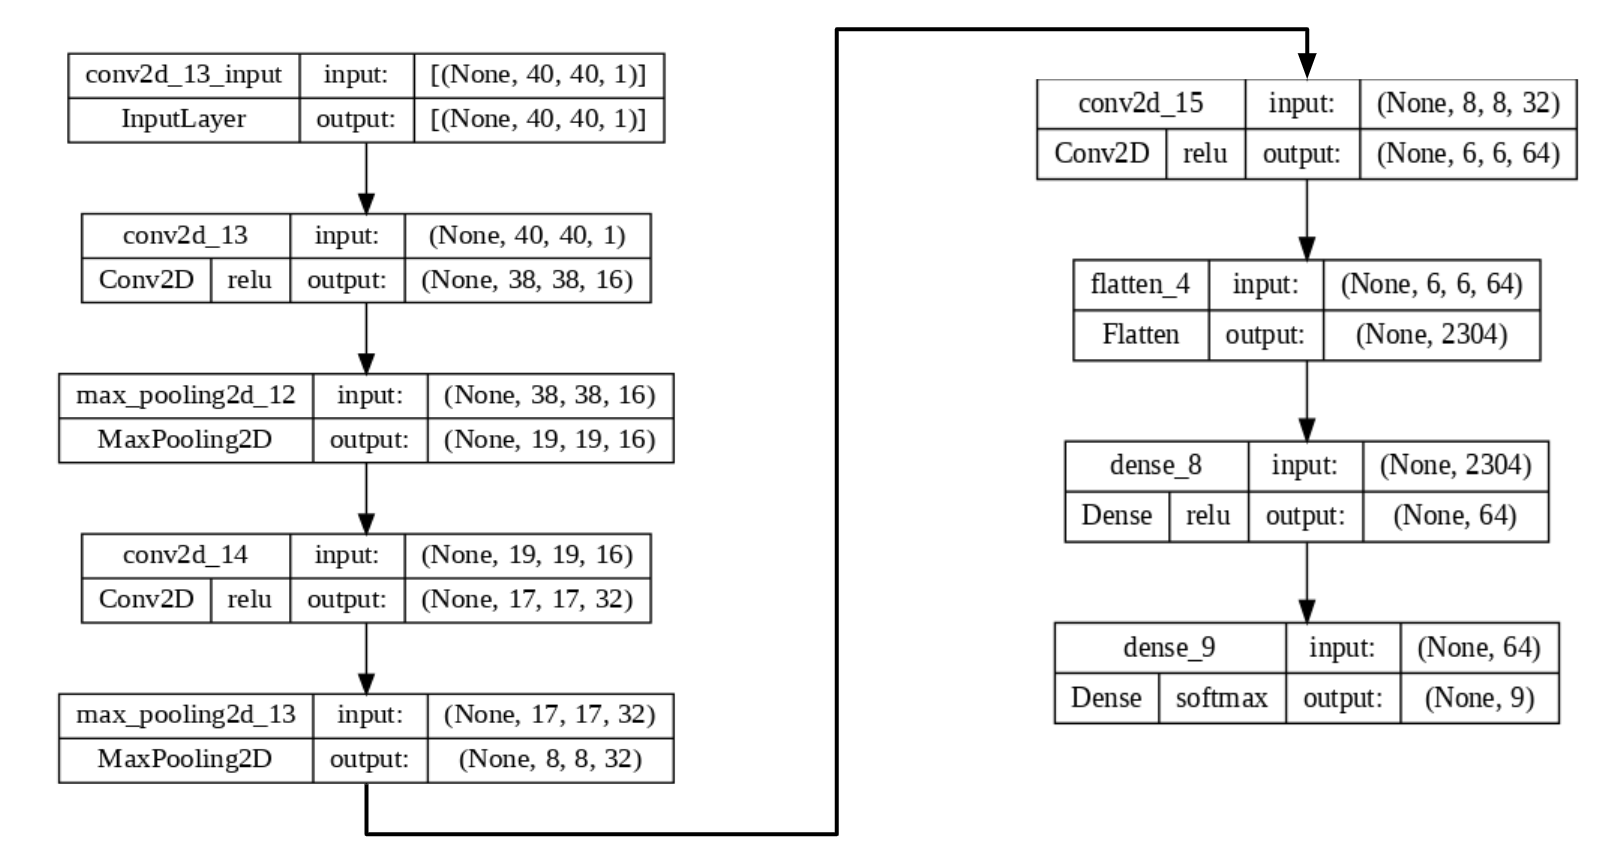
\includegraphics[width=0.8\textwidth]{Images/Perf_Eval/NN_Architecture.png}
    \caption{CNN\_Model\_1 Network Architecture}
\end{figure}

\noindent The model architecture (refer to Figure 3.8) consists of a sequential arrangement of layers. It begins with a convolutional layer, utilizing 16 filters of size 3x3 and employing the ReLU activation function. This layer processes input images with dimensions of 40x40 pixels and a single color channel. Subsequently, a max-pooling layer is applied to downsample the feature maps.

\clearpage

\noindent The next convolutional layer incorporates 32 filters of size 4x4 and also uses the ReLU activation function. However, there is no max-pooling layer following this convolutional layer, which helps preserve spatial information in the feature maps. The flattening layer is then employed to transform the multidimensional feature maps into a flat representation.\\

\noindent Two dense layers are added next. The first dense layer consists of 64 units and uses the ReLU activation function. The final dense layer has a number of units equal to the number of output classes and employs the softmax activation function, providing probability distribution predictions.\\

\noindent Moreover, the model is compiled using the Adam optimizer. The loss function used is sparse categorical cross-entropy, suitable for multi-class classification tasks. The metric used for evaluation is accuracy, measuring the performance of the model during training and testing. This architecture, with the absence of a pooling layer after the last convolutional layer, is designed to effectively process and classify images with high accuracy.\\

\noindent In conclusion, the process of marks extraction from table cells involves the utilization of a table extraction algorithm and a CNN model. The algorithm enables the identification and isolation of individual cells within the table, allowing for the extraction of marks from each cell. The CNN model plays a vital role in accurately classifying and interpreting the marks within the cells. The inclusion of exception checking within the algorithm ensures error handling and robustness in cases where the expected number of cells is not detected. By incorporating these components and mechanisms, the automated marks extraction system achieves reliable and accurate results, facilitating streamlined data processing and analysis in educational assessment processes.

\subsection{Classification}

\noindent The marks extraction process in the system employs a Convolutional Neural Network model for classification. The CNN is trained to categorize input images into nine classes, representing numerical values from 0 to 7, and an additional class for empty cells. It classifies the numerical equivalent of image cells or identifies them as null if empty.

\clearpage

\noindent During the prediction phase, the CNN model takes an input image and processes it through its layers. By analyzing the image features and extracting meaningful representations, CNN makes accurate predictions and classifications.

\noindent To ensure the correct sequence of marks, the extracted predictions are stored in a dictionary structure. Each dictionary key corresponds to a table-detected cell, ensuring that the predicted cell values are associated with their respective positions within the table. This maintains the integrity and accuracy of the marks extraction process.

\noindent By predicting all cell values before receiving the next input, the CNN model ensures efficient and consistent processing. This approach swiftly extracts and stores the predicted marks in their corresponding positions, facilitating streamlined data management and subsequent analysis.

\noindent  Thus the classification of the system is achieved through a CNN model, effectively categorizing image cells into numerical classes or identifying them as null. The trained representations of the model enable accurate classification, and the extracted marks are efficiently stored in a dictionary, preserving their positions within the table. 

\noindent This methodology ensures the efficiency and accuracy of the system in the extraction of marks, making it a reliable and valuable tool for educational institutions.

\subsection{Data Post-processing}

\noindent After obtaining the classification result in the form of a dataframe, the first crucial step in the data post-processing phase involves removing the first column of the dataframe, this is done to remove the column that contains the possible sub-sections(A, B, C) corresponding to each question numbers(1A, 1B, 1C, ..., 12B, 12C). This column removal will give the marks which is the essential thing need from the table and it simplifies the data for further processing.

\noindent Once the dataframe is appropriately cleaned, the next step is to flatten the resultant dataframe column-wise. This process allows to collect the marks corresponding to each sub-section of a question (if they exist). The final one-dimensional array is integrated into the marks dictionary, with respect to the dictionary keys(where keys represent the question number with sub-section alphabet).

\clearpage

\noindent This ensures that the extracted marks are well-organized within the dictionary. Each image inputted into the system will go through this process, consolidating the extracted marks from multiple answer scripts into the marks dictionary.

\noindent After processing all the images, the marks dictionary will contain the scores obtained by students in each question. However, it may also include columns with no marks (for questions without sub-sections). To remove these empty columns, the dictionary is converted to a dataframe for easy processing then the empty columns are dropped using appropriate code to make the output look similar to what is manually created by humans. For convenience in editing, two empty columns named 'Name' and 'Roll Number' will be added to the right side of the dataframe, so that the teachers can add the name and roll number data seamlessly.

\noindent The final dataframe is converted to CSV format and this file will have marks that are scored by the students in each question, or in other words this output is what the teachers create in 4-6 hours using their valuable time. The CSV format provides an easy-to-read way of storing the extracted marks, making it simple to use with other applications and allowing for further analysis and edits if needed. Successfully completing the data post-processing phase signifies achieving the objectives of the project- developing an efficient and effective system that automates the mark extraction process from answer scripts, significantly reducing workload of teachers.

\section{Summary}

% \vspace{0.5mm}

\noindent
The proposed system which is discussed in detail performs very efficiently in comparison with existing systems. The computation time of the proposed system varies from computer to computer as the specifications of the computer in use determine the difference in computation time when compared to other computers. Based on calculations, the proposed system is capable of achieving an average time of 18.5 milliseconds for the classification of images. Also, the proposed system also exhibits the ability to process 5 samples of answer scripts in 13 seconds, which pushes the advantage of using the system even more.